\section{Method RQ 3 - Collection geodata of rollator movements and analysis}\label{rq2b}
The data collection and pre-processing per sensor used in this research will be explained in the next sections per sensor. The different sensors make use of different time zones or geographic systems, therefore some general pre-processing steps had to be conducted to standardize all the files in order to compare them in the end. 

\subsection{Data Collection - GPS }
Several sensors were used for measuring GPS, varying in its details and specifications. The reason several ways to measure location were used is because not all the devices were available all the time. 

\begin{description} 
\item[Garmin Summit]
For the rollator loop the Garmin Summit was used with the following specifications:
\begin{itemize}
\item Time zone: UTM
\item Projected Coordinate System: WGS84
\end{itemize}
\end{description}

\begin{description}
\item[GPS Geotracker ]
On the smart phone the application GPS Geotracker was used. Version: 3.0.3 from 23 July 2015 Author: Ilya Bogdanovisch. This resulted in the following specifications:
\begin{itemize}
\item Time zone: UTM
\item Projected Coordinate System: WGS84
\end{itemize}
\end{description}

\begin{description}
\item[Leica GNSS RTK]
For more precise location measurements the Leica system was attached to the Measurement Rollator. Though, only one Leica system was available and it was to heavy to attach to an elderly's rollator. The following specifications:
\begin{itemize}
\item Time zone: UTM
\item Projected Coordinate System: WGS84
\end{itemize}
\end{description}

The Leica is much more precise then the Garmin or the GPS tracker on the smart phone. But when the Leica was not available, the other two methods still gave a good reference as were the route was. 

\subsection{Data Pre-processing - GPS }
Figure \ref{gpspp} shows all pre-processing steps that are applied to all location datasets. First the files are imported into Arc-map, creating point features. From from GPX or KLM file. When necessary, they were transformed from WGS1984 to RD new. The time attribute was edited all data contained the format YYYY-mm-dd HH:MM:SS.OOO and was transformed to time zone CET. The Track Analyst tool was used for computing difference in time, speed and course between every GPS point. The settings used are: 
\begin{itemize}
 \item First to second point
 \item Meters, Seconds, Meter per seconds and Degrees
\end{itemize}
Eventually, the dataset were manually edited to delete the start and end points, if necessary. To exclude the waiting time before the actual walking, and the waiting at the end to turn the devices off. 

\begin{figure}[hb]
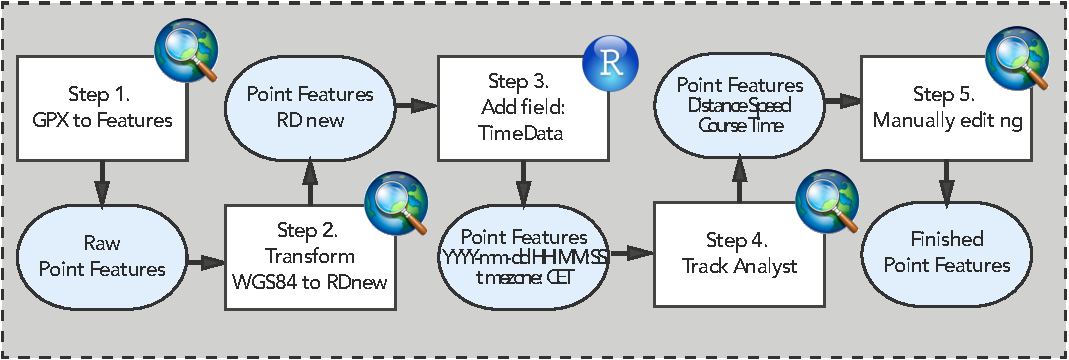
\includegraphics[width=\textwidth]{img/M_preprocessingGPS.pdf}
\centering
\caption{GPS pre-processing flowchart}
\label{gpspp}
\end{figure}

\subsection{Data Collection - Accelerometer}
We used a Samsung Galaxy Core GT-I8260 smart phone which was available at the conducting faculty. With the application; Accelerometer Physics toolbox accelerometer to extract the 3-axis acceleration data on the X, Y and Z axis and the total acceleration called g-force. Physics Toolbox Accelerometer proved to be the best option for extracting the data, for it is easy to use, can store the data in a csv file, with current clock time, time stamp and saves it on the local storage of the phone. It does not require a constant internet connection, and was free for use. Also no knowledge on any pre-programming to read the sensors was required. Some of the other application alternatives considered are: Accelerometer Monitor from Mobile Tools, Accelerometer Monitor from Keuwlsoft Tools, and the AcMeter. Their specifications and reasons why not used, can be found in Annex \ref{Aapps}. 

During all measurements, the smart phone will always be placed horizontally on the Rollator. This means the $z$-axis is pointing down, and will correlate most with movements up and down. The x-axis will be pointing sideways and the y-axis front and back. Acceleration of walking speed will be seen in the $y$-axis. While turns will be seen in the $x$-axis. See figure \ref{setup}.
\begin{figure}[t]
\includegraphics[width=\textwidth]{img/M_RollatorSetup.pdf}
\centering
\caption{ Graphical representation of the direction of the axis of the accelerometer on the rollator. \label{setup}}
\end{figure}


\subsubsection{Application version change}
Several versions of the application were used, as the developer updated the app meanwhile. \footnote{Information provided by Chrystian Vieyra, developer of the Physics Toolbox Applications. In e-mail conversation 26-10-15. }
In September 2015 version 1.2.9 was active. On September 9th the version available was 1.3.6. Though, the smart phones used, were not always attached to the internet, and so version 1.29. was used in the beginning. This resulted into failed experiments for there was no wake lock, which keeps the device awake even if the screen turns off while the record button has been pressed. So the app was put to sleep during the measurements. Test rides on a bike were conducted but the gaps of missing data seemed to happen when large bumps occurred in the road and the conducting researcher kept the screen awake more often by touching the smart-phone more often. 

Later measurements were taken with version 1.3.6 and 1.3.7, which did continue the app measuring when the screen was in sleep mode. The only difference between version 1.3.6 and 1.3.7 is a spelling mistake and the graphic layout of the record button.


\subsection{Data Pre-processing - Accelerometer}
The accelerometer dataset contains the following specifications:
\begin{itemize}
\item Time zone: CET. Same as the smart phone settings. 
\item CSV time stamp: clock time in milliseconds
\item No location
\end{itemize}

The measurements resulted in dataset with per feature :
\begin{equation} 
	F_{(t)} = [A_{x}, A_{y}, A_{z}, A_{m}] 
\end{equation}
With $A_{x}$ as the $x-axis$ acceleration
$A_{y}$ as the $y-axis$ acceleration
$A_{z}$ as the $z-axis$ acceleration and
$A_{m}$ as the total acceleration.

The total acceleration or g-force is supplied by the application: It is the total acceleration vector of the 3 axis combined. When tested, the calculated $A_{m}$ is equal to the g-force provided by the application. It will be referred to as $A_{m}$ or total acceleration, for G-force can be a confusing concept. It can be calculated by:

\begin{equation}
A_{m} = \sqrt {{A_{x}}^{2} + {A_{y}}^{2} + {A_{z}}^ {2}}
\end{equation} For each time series $A_{i}$ , with $i = {x, y, z}$ 

With cross correlation between the several features, we can detect which feature best represents the walk characteristics. $A_{m}$ is a representative parameter which includes the gait acceleration (Y-axis), the vertical acceleration (Z-axis) and the lateral acceleration (X-axis).~\cite{Weiss2014} By doing a cross correlation with the Z-axis and the X and Y axis a similarity between the lateral acceleration, mostly caused by the surface, and the gait acceleration is detected. The cross correlation of the $x$ and $z$ axis is expressed by:

\begin{equation}
Corr_{z,x} = \sum z(n)x(n-1) %blablabla wat doe ik hiermee? 
\end{equation}

Accelerometer output ranged between the normalized range of -2 to 2. Assumed is that the value of 1 means equal to 1 times the gravitational force: 9.81 $m/s^2$ and the value of 0 means no force pulling, so the sensor is flat. The developer stated, that these normalized values differ per type of smart phone.\footnote{Information provided by Chrystian Vieyra, developer of the Physics Toolbox Applications. In e-mail conversation 26-10-15. }

The application contained several settings, which were not described in the application nor on-line. Therefore some sample test were conducted to gain some basic information about the application values and settings. The application had four record interval settings, Normal, UI, Game and Fast. By placing the phone for a while on the table with the different settings the following information was found about the sample frequency of these settings: 

\renewcommand{\arraystretch}{1.5}

\begin{table}[h]
\caption{Sample frequency of the different settings.}
\label{samfreq}
\centering
\begin{tabular}{|p{91pt}|p{91pt}|p{91pt}|p{91pt}|} 
\hline 
 Setting & Points per sec \newline (exact) & Points per sec \newline (approx.) & Periodicity \newline (1/(points per sec))\\
\hline
NORMAL & 4.6 & 5 & 0.2 \\
UI & 11.9 & 10 & 0.1 \\
GAME & 49.6 & 50 & 0.02 \\
FAST & 99.4 & 100 & 0.01 \\
\hline
\end{tabular}
\end{table}

This means that with an average walking speed of 1.3$m/s$ the distance between the measured points will be, 26$cm$ for NORMAL sample frequency, 13$cm$ for UI, 2.6$cm$ for GAME and 1.3$cm$ for FAST sample frequency. 
For further calculations the setting NORMAL is used. This because an interval of 26 cm seams sufficient and the data set will be not too large in size to handle. 

\subsubsection{Sensor errors}
Because the accelerometer sensor is not calibrated and the quality is unknown, it can contain random errors (caused by the accuracy limit of the measuring instrument) or systemic error (caused by incorrect calibration of the measuring instrument). 
By placing the smart phone flat on a table, laying still for several hours, an indication can be given of the sensors offset. This means the z-axis is pointing down and also contains one time the gravitational force pulling it down. Resulting in numbers around 1. The x and y axis are pointing to the side and front/back. Being flat and resulting in numbers around 0.

The following sensor errors were found with setting NORMAL for every axis:

\renewcommand{\arraystretch}{1.5}
\renewcommand{\tabcolsep}{0.2cm}
\begin{table}[h]
\centering
\caption{Average error per axis. Sample frequency 5 per sec (NORMAL)}
\label{averageerror}
\begin{tabular}{|p{56.6pt}|p{56.6pt}|p{56.6pt}|p{56.6pt}|p{56.6pt}|p{56.6pt}|} 
\hline
\multicolumn{2}{|c|}{SAM 3} & \multicolumn{2}{|c|}{SAM 4} & \multicolumn{2}{|c|}{SAM 5} \\
\hline
\multicolumn{2}{|c|}{Average error from 0} & \multicolumn{2}{|c|}{Average error from 0} & \multicolumn{2}{|c|}{Average error from 0} \\ 
\hline
$\xi_{A_x}$ & -0.04 &$\xi_{A_x}$ & -0.05 &$\xi_{A_x}$ & -0.03 \\
$\xi_{A_y}$ & 0.03 & $\xi_{A_y}$ & 0.06 & $\xi_{A_y}$ & 0.05 \\
$\xi_{A_z}$ & 1.01 & $\xi_{A_z}$ & 1.02 & $\xi_{A_z}$ & 1.03 \\
$\xi_{A_m}$ & 1.02 & $\xi_{A_m}$ & 1.02 & $\xi_{A_m}$ & 1.03 \\
\hline
\end{tabular}
\end{table}

These average errors $\xi_{A_x}$ , $\xi_{A_y}$, $\xi_{A_z}$ and $\xi_{A_m}$ are extracted from all measured Accelerometer time series per smart phone. 

\subsection{Assigning location to accelerometer data with GPS}\label{locationassigning}
For reference, the accelerometer data can be linked to the location by using the time-stamp of the accelerometer and the GPS points. With the time stamp, the first GPS point before and the first GPS point after that time is taken. Because the time difference between the first GPS point and the unknown accelerometer point is known and the speed $(s)$ between the GPS points, the distance$(d)$ and so location$(x,y)$ of the unknown accelerometer point is calculated. 

\begin{figure}[H]
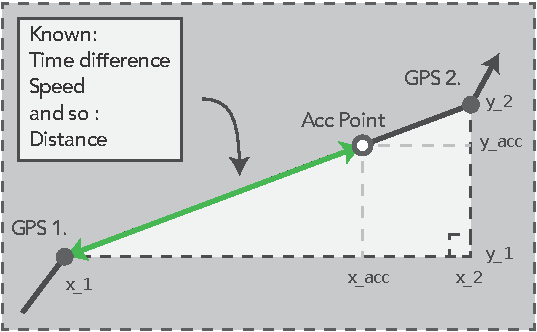
\includegraphics[width=\textwidth]{img/M_location_calc.pdf}
\centering
\caption{Graphical explanation of changepoint location calculations \label{cpcalc}}
\end{figure}

With coordinates ($x_{1}, y_{1}$) and ($x_{2}, y_{2}$) in RDnew as the known first and second GPS point, respectively. 

The distance between $(x_{1}, y_{1})$ and $(x_{2}, y_{2})$ is calculated by:
\begin{equation}
d_{1,2} = \sqrt {(y_{1}-y_{2})^2 + (x_{1}-x_{2})^2 }
\end{equation}

Then, the distance between GPS point 1 $(x_{1}, y_{1})$ and the un-located accelerometer point $(x_{Acc}, y_{Acc})$ is calculated with:
\begin{equation}
d_{1,Acc} = s * time difference((x_{1}, y_{1}) - (x_{Acc}, y_{Acc}))
\end{equation}

The unknown $x$ coordinate of the accelerometer point is calculated with:
\begin{equation}
x_{Acc} = x_{1} + \frac{d_{1,cp}}{d_{1,2}} * (x_{2} - x_{1})
\end{equation}

And the unknown $y$ coordinate of the accelerometer point is calculated with:
\begin{equation}
y_{Acc} = y_{1} + \frac{d_{1,cp}}{d_{1,2}} * (y_{2} - y_{1})
\end{equation}

Now we can add the location specific data to the changepoints, the speed($S$) extracted from the track GPS points and the AHN values, height and slope. Resulting in a feature per observation of:

\begin{equation} 
	F_{(t)} = [A_{x}, A_{y}, A_{z}, A_{m}, s, height, slope] 
\end{equation}

\subsection{Data Collection - Movie material}
Most walks were recorded on film, for reference aid. This was done with either a go-pro, flip camera or with the smart phone camera. Pointed at the direct surface in front of the rollator. The images are not used for calculations, solely for reference backup. 

\subsection{Analysis - Mapping irregular surfaces with an Accelerometer}
Several test were conducted with the Measurement Rollator on different surfaces. To see if the vibrations of the rollator are more fierce on surfaces with a more irregular surfaces. Indicating more surface hindrance and so more energy is needed for the rollator user. The assumption is, that the vibrations caused by surface hindrance can be measured through the variance of the z-axis acceleration. We used the Accelerometer (Physics Toolbox version 1.3.7) and the Garmin to record GPS. The goal was to walk with an average walking speed of $4.7 km/h$ average between $3.2$ and $6.2 km/h$. This is the walking speed found from literature and own research. Though, while walking it felt quite fast. So the walking speed was kept around 4 km/h as best as possible. The researcher walked herself with the rollator over different surfaces. Each a distance of around $20m$. All the pavement surfaces structures shown in image \ref{surfaceimg} were tested. Asphalt or tarmac, brick paving, tiles, gravel, grass and a smooth concrete surface inside was measured. 

\begin{figure}[p]
\includegraphics[width=\textwidth]{img/M_All_surfaces.pdf}
\centering
\caption{Image of every measured surface \label{surfaceimg}}
\end{figure}

\begin{figure}[p]
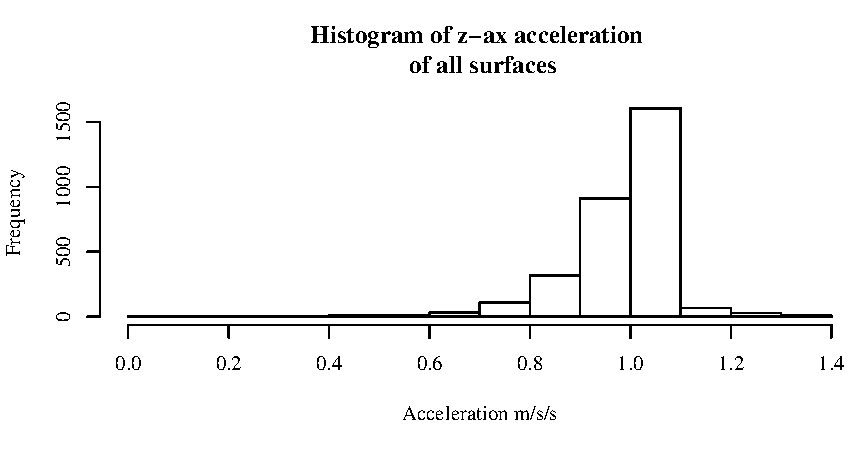
\includegraphics[width=\textwidth]{img/M_Histogram_all_surf.pdf}
\centering
\caption{Histogram of all surfaces $z$-axis acceleration \label{hist}}
\end{figure}

\subsubsection{Statistics}
By providing the descriptive statistics of the accelerometer output as a normal distribution, the differences in the vibrations on different surfaces can be explained. The data is approaching a normal distribution as can be seen in the example histogram of all the surfaces combined, with a mean around 1.(~\ref{hist}) Vibration goes into both directions so the mean will not show a surface specific outcome and will not differ much between the different surfaces. See table~\ref{surfacehindrance} in the results. The variability shows better how rough the surface is. Therefore the variability is used, or the standard deviation together with the 5-number summary to create box plots. Including, the minimum, maximum, median and first and third quantile. To show a better understanding of the effect of the surface on the vibrations on the rollator. The formula for the mean variance and standard deviation:

\textbf{Mean:} 
\begin{equation}
Mean A_{z} = \frac{\sum_{k=1}^n A_{z}}{n}
\end{equation}

\textbf{Variance:}
\begin{equation}
\sigma^2 = \frac{\sum_{k=1}^n (A_{z}- mean(A_{z}))^2}{n-1}
\end{equation}

\textbf{Standard deviation:}
\begin{equation}
\sigma = \sqrt \frac{\sum_{k=1}^n (A_{z}- mean(A_{z}))^2}{n-1}
\end{equation}

\subsubsection{Comparison with Matthews et al. (2003)}
In Matthews et al. (2003)~\cite{Matthews2003} a reference score for hindrance of specific surfaces is provided. Shown in table~\ref{hindrance}.
Small test were conducted measuring surface hindrance for wheelchair users, aiming at surface type and quality for mobility. Six common urban surfaces were tested: concrete, paving, tarmac, brick, grass and gravel. A wheelchair with occupant was pushed down a small ramp the distance rolled provides an measure for rolling resistance.~\cite{Matthews2003}
These values will be used as a reference, to see if the measured vibrations of the Accelerometer correlate. Because the reference numbers are relative, also the measured outcome is recalculated to a relative factor. Taking the most smooth surface as factor 1 and calculating the rest of the surfaces from this. See results in figure~\ref{comparefig} for a comparison of the values of Matthews and the calculated factors. 
 % figure comparison factors measured and given 4.3

\begin{table}[hb]
\caption[Relative hindrance scores of surfaces]{Relative hindrance scores of surfaces, low scores represent levels of least hindrance~\cite{Matthews2003} \label{hindrance}}
\centering
\begin{tabular}{|l|l|l|l|l|l|}
	\hline
	Concrete & Paving & Tarmac & Brick & Grass & Gravel\\
	\hline
	1 & 1.2 & 1.3 & 1.6 & 6 & 8 \\
	\hline
\end{tabular}
\end{table}